\documentclass{IEEEcsmag}

\usepackage[colorlinks,urlcolor=blue,linkcolor=blue,citecolor=blue]{hyperref}
\expandafter\def\expandafter\UrlBreaks\expandafter{\UrlBreaks\do\/\do\*\do\-\do\~\do\'\do\"\do\-} \usepackage{upmath,color} \usepackage[super]{cite} \usepackage{tikz} \usetikzlibrary{arrows.meta,positioning,fit,calc}

%%  -  -  -  -  -  -  -  -  -  -  -  -  -  -  -  -  -  -  -  -  - 
%% Author notes (in Italian, red). Set \shownotestrue to hide them
%% before submission. All of them must be resolved by the authors.
\newif\ifshownotes \shownotestrue
\newcommand{\nota}[1]{\ifshownotes{\color{red}\,[\textbf{NOTA:} #1]}\fi}
\newcommand{\tbd}{\ifshownotes{\color{red}\textbf{TBD}}\else{ - }\fi}
%%  -  -  -  -  -  -  -  -  -  -  -  -  -  -  -  -  -  -  -  -  - 

\jvol{XX}
\jnum{XX}
\paper{8}
\jmonth{Month}
\jname{IEEE Software}
\jtitle{IEEE Software}
\pubyear{2027}

\setcounter{secnumdepth}{0}

\begin{document}

\sptitle{Theme Article: Next-Generation Software for Smart, Resilient, and Sustainable Cities}

\title{Open Tools for Catching Stereotypes in Smart City LLM Services}

\author{Roberto Vergallo}
\affil{Pegaso University, Naples, 80132, Italy}

\author{Danilo Giovannico}
\affil{University of Salento, Lecce, 73100, Italy}

\author{{L}uca Lotti}
\affil{ZeroDD S.c.a r.l., Lecce, 73100, Italy}

\author{{L}uca Mainetti}
\affil{University of Salento, Lecce, 73100, Italy}

\markboth{THEME ARTICLE}{THEME ARTICLE}

\begin{abstract}\looseness-1
Smart city services increasingly answer residents through large language models (LLMs), and these models can repeat stereotypes about gender, ethnicity, religion, and occupation. We package three open, reproducible tools for delivery teams: a unified three-label corpus, a dual-axis evaluation protocol that reports detection quality (macro-F1) and preference fairness (adapted StereoSet iCAT) separately, and a compact released classifier (VAN) plus six integration patterns for LLM pipelines.
\end{abstract}

\maketitle

\chapteri{C}ities are putting large language models (LLMs) behind the services residents use every day. A municipal chatbot answers questions about waste collection and school enrollment, an assistant drafts replies to complaints sent through the city portal, and public employment offices test tools that summarize r\'esum\'es or write job ads. These services reach everyone, including the residents who are already most exposed to discrimination. When the model behind them repeats a stereotype, it is the city that speaks.

Social sustainability asks that development leave no one behind, a principle written into the United Nations 2030 Agenda.\cite{un2030} For software teams, the principle becomes a quality requirement: a city service should give every resident the same quality of answer, whatever their gender, origin, religion, or occupation. European law points the same way. The AI Act classifies as high-risk the AI systems that public authorities use to evaluate access to essential public services and benefits.\cite{aiact} A chatbot outside that category still carries legal and reputational risk when it produces discriminatory text.

Most teams that build these services are not specialists in natural language processing. They integrate a hosted or open-weight model, write prompts, and connect the result to city data. Research on fairness in LLMs is large,\cite{gallegos2024} but it is spread across benchmarks with different label schemes and across metrics designed for language models, so it is hard to turn into tests that a delivery team can run.

This article packages our work on stereotype detection into three tools for such teams. The first is an open labeled corpus with one label scheme. The second is a dual-axis evaluation protocol---macro-F1 for detection and an adapted StereoSet iCAT for preference fairness---together with a compact open classifier (VAN) released under that protocol so teams can reproduce the product numbers and the matched ablations. The third is a set of six patterns for wiring the classifier into an LLM pipeline.

\section{WHAT DELIVERY TEAMS OFTEN MISS}

Researchers measure stereotypes in language models with public benchmarks. Two of the most used are StereoSet,\cite{nadeem2021} a crowdsourced collection of short contexts, each followed by a stereotyped, an anti-stereotyped, and an unrelated continuation, and CrowS-Pairs,\cite{nangia2020} a set of sentence pairs that differ only in the social group they mention. Work on these benchmarks offers two lessons that rarely reach day-to-day delivery work: a set of facts about how stereotypes show up in LLM output, and a set of metrics that go beyond the accuracy figures teams already track.

\subsection{Overlooked Facts}

Four findings are familiar to researchers and less visible to delivery teams.

\begin{itemize}
\item[{\ieeeguilsinglright}] {\it Fluent output can still be biased.} Grammar checks, relevance scores, and user ratings do not catch a stereotype phrased politely. The authors of StereoSet found that the stronger language models in their study also showed stronger stereotypical preferences.\cite{nadeem2021}

\item[{\ieeeguilsinglright}] {\it A reversed stereotype is still a stereotype.} Both benchmarks pair each stereotyped sentence with an ``anti-stereotyped'' one. In StereoSet, the context ``Many people live in Ethiopia'' is followed either by ``The people are very thin and good at distance running'' or by ``The people are fat and unathletic.'' Both sentences assign a trait to a whole nationality. A city service should avoid both, so a model must never be rewarded for producing the second one.

\item[{\ieeeguilsinglright}] {\it Benchmarks have noise and a cultural viewpoint.} An audit of four fairness benchmarks, including StereoSet and CrowS-Pairs, found items that are ungrammatical, that express no stereotype, or that target the wrong group.\cite{blodgett2021} Most benchmarks also encode stereotypes from the United States, in English. A city in southern Italy that serves Italian speakers and newly arrived residents must localize them.

\item[{\ieeeguilsinglright}] {\it A judge that trains a model cannot also grade it.} When a classifier serves as the reward for fine-tuning, the LLM learns to satisfy that classifier, including its blind spots.\cite{gao2023} Scores from the same classifier then overstate progress.
\end{itemize}

\subsection{Metrics Beyond F1}

A stereotype detector must be judged on two axes, and they are separate measurements. The first is detection quality: does it label sentences correctly? The standard measure is the macro-averaged F1 score, computed overall and for each bias type, together with accuracy, precision, and recall. The second is fairness of preference: when the detector sees a stereotyped and a counter-stereotyped version of the same sentence, does it treat them alike? A guardrail that catches ``women are bad drivers'' but lets ``men are bad drivers'' through applies a double standard, even when its F1 score is high.

StereoSet measures the second axis with the idealized Context Association Test (iCAT) score.\cite{nadeem2021} Its candidate sentences come in triplets that share a context: one stereotyped, one counter-stereotyped, and one unrelated. In the original benchmark, preferences are derived from a language model's likelihoods over candidates. We keep the same algebraic form of iCAT but adapt the preference rules to a three-class classifier that scores each candidate independently (not as a joint LM over the triplet). Let $p_{\mathrm{stereo}}$, $p_{\mathrm{anti}}$, and $p_{\mathrm{unrel}}$ be the softmax probabilities for labels 0/1/2 on one candidate. Over $N$ candidates,
\begin{equation}
\begin{aligned}
\mathit{lms}
  &= 100\cdot\frac{1}{N}\sum_{i=1}^{N}
     \mathbf{1}\!\bigl[
       \max(p_{\mathrm{stereo}}^{(i)}, p_{\mathrm{anti}}^{(i)})
       > p_{\mathrm{unrel}}^{(i)}\bigr],\\
\mathit{ss}
  &= 100\cdot\frac{1}{N}\sum_{i=1}^{N}
     \mathbf{1}\!\bigl[
       p_{\mathrm{stereo}}^{(i)} > p_{\mathrm{anti}}^{(i)}\bigr],\\
\mathit{iCAT}
  &= \mathit{lms}\cdot\frac{\min(\mathit{ss},\,100-\mathit{ss})}{50}.
\end{aligned}
\end{equation}
An ideal detector has $\mathit{lms}=100$ and $\mathit{ss}=50$, which gives $\mathit{iCAT}=100$. A detector that always prefers one stereotype direction scores zero, however fluent its labels look. We compute $\mathit{lms}$, $\mathit{ss}$, and $\mathit{iCAT}$ separately on intersentence items (input $=$ context concatenated with the continuation) and on intrasentence items (filled sentence alone), then report
\begin{equation}
\mathit{iCAT_{avg}}
  = \tfrac{1}{2}\bigl(
      \mathit{iCAT}_{\mathrm{inter}}+\mathit{iCAT}_{\mathrm{intra}}
    \bigr).
\end{equation}
This adapted iCAT is a preference-fairness probe for the classifier; it is not a drop-in replica of the original LM-based StereoSet score. Controlled checks match the intended extremes: if every candidate has $p_{\mathrm{stereo}}>p_{\mathrm{anti}}>p_{\mathrm{unrel}}$, then $\mathit{ss}\to 100$ and $\mathit{iCAT}\to 0$; if always $p_{\mathrm{anti}}>p_{\mathrm{stereo}}>p_{\mathrm{unrel}}$, then $\mathit{ss}\to 0$ and $\mathit{iCAT}\to 0$; if meaningful classes dominate the unrelated class and $\mathit{ss}\approx 50$, then $\mathit{iCAT}\approx\mathit{lms}$.

Detection quality (F1) and preference fairness (iCAT) use \emph{related but different} StereoSet-derived resources, on purpose. iCAT is computed on the official StereoSet splits, where the third candidate is the benchmark's ``unrelated'' continuation. Macro-F1 is \emph{not} computed against that official \texttt{gold\_label}, because unrelated text is not the same as the fluent \emph{neutral} / no-association class (label~2) used in our unified three-label scheme. Instead, F1 uses a modified multiple-choice release of StereoSet contexts (\texttt{stereoset\_select\_options}): each item still has a stereotyped and a counter-stereotyped option (labels 0 and 1), but the meaningless unrelated option is replaced by a fluent neutral continuation (label~2), consistent with the corpus of Tool~1. Each option is scored as \texttt{context [SEP] sentence}; we compare $\arg\max$ predictions (no confidence or abstention gates) to those construction labels on a \emph{leak-free} select-options set (150 prompts, 450 options; Table~\ref{tab:results}), never to a \texttt{label\_predicted} field written by the same model. The older full select-options test split (322 prompts, 966 options) has residual exact-string overlap with the development pool and is \emph{not} the F1 resource used in Table~\ref{tab:results}.

The two axes must be read together and per bias type, because an average across groups can look excellent while one group is served poorly. When we refer to inter-group disparity we mean a diagnostic gap $\Delta_{\mathrm{iCAT}}=\max_g\mathit{iCAT}_g-\min_g\mathit{iCAT}_g$ (and likewise for F1), not a training objective.

\section{TOOL 1: AN OPEN CORPUS WITH ONE LABEL SCHEME}

Each public benchmark labels bias in its own way. We merged four sources into one corpus where every sentence carries one of three labels (Table~\ref{tab:corpus}). Label 0 (\emph{stereotyped}) and label 1 (\emph{counter-stereotyped}) mark sentences that associate a social group with a trait, in the conventional or in the reversed direction. Label 2 (\emph{no association}) marks sentences that make no such association.

\begin{table*}
\caption{Sources of the corpus and mapping to our labels. The initial unified corpus has 55,817 sentences: 18,591 stereotyped (label 0), 18,387 counter-stereotyped (label 1), and 18,839 with no association (label 2). For intersentence items, the context and the continuation are joined with a separator token.}
\label{tab:corpus}
\tablefont
\begin{tabular*}{\textwidth}{@{\extracolsep{\fill}}p{58pt}<{\raggedright}p{105pt}<{\raggedright}p{125pt}<{\raggedright}p{120pt}@{}}
\toprule
Source & Bias dimensions & Mapping to our labels & Enrichment\\
\colrule
WinoBias\cite{zhao2018}
  & Gender in occupations
  & Pro-stereotypical $\to$ 0; anti-stereotypical $\to$ 1
  & Up to 10 synonym variants per sentence\\[3pt]
CrowS-Pairs\cite{nangia2020}
  & Race, gender, religion, and six more types
  & For each pair, \texttt{sent\_more}/\texttt{sent\_less}
    labeled 0 or 1 by \texttt{stereo\_antistereo}
    (stereotypical side $\to$ 0;
     counter-stereotypical $\to$ 1)
  & Synonym variants; near-duplicates removed\\[3pt]
StereoSet\cite{nadeem2021}
  & Gender, profession, race, religion
  & Stereotype $\to$ 0; anti-stereotype $\to$ 1;
    regenerated neutrals $\to$ 2
  & Synonym variants; neutral continuations generated
    for each context $\to$ 2\\[3pt]
Tatoeba
  & None (everyday sentences)
  & English sentences that name no group $\to$ 2
  & Duplicates and very short sentences removed\\
\botrule
\end{tabular*}
\end{table*}

WinoBias\cite{zhao2018} contributes sentences about occupations and gendered pronouns, from all four of its subsets. CrowS-Pairs contributes its sentence pairs with their bias type; labels follow the CrowS \texttt{stereo\_antistereo} field (stereotypical side~$\to$~0, counter-stereotypical~$\to$~1), so \texttt{sent\_more} is not always label~0. StereoSet contributes both of its formats: intrasentence items, where the candidates differ in a single word, and intersentence items, where a shared context is followed by three different continuations. Tatoeba (\url{https://tatoeba.org}), a collection of short sentences written by volunteers for translation, provides ordinary text that names no group, so the classifier learns that most messages are harmless.

Public benchmarks are small, so we enriched them with automatic steps that any team can rerun. Using part-of-speech tags from NLTK, we replaced nouns, adjectives, and adverbs with WordNet synonyms to create lexical variants. Every new sentence passed a grammar check by a BERT classifier fine-tuned on the Corpus of Linguistic Acceptability (CoLA), and failing sentences were dropped. The unrelated StereoSet continuations are often nonsensical, so we replaced them with neutral continuations generated by GPT-2 from the same context and filtered with the same grammar check. We then removed duplicates by hashing, normalized spacing and punctuation, and filtered toward a length band of roughly 3 to 512 tokens (a small residue of shorter sentences remains). All records share one JSON form with three fields: sentence, bias type, and label.

The initial unified corpus is approximately balanced across labels (see the caption of Table~\ref{tab:corpus}). By bias type it contains 12,760 sentences on gender, 11,885 on race and color (Table~\ref{tab:corpus-counts}: \texttt{race}~$9{,}340$ plus \texttt{race-color}~$2{,}545$), 8,091 on profession, and 1,176 on religion, plus smaller groups on socioeconomic status, nationality, age, sexual orientation, physical appearance, and disability; 18,839 sentences carry no bias type.

To keep a held-out preference benchmark, we removed from the unified corpus any sentence that exactly matched StereoSet test material after string normalization. From the initial 55,817 sentences we dropped 5,408 such examples, leaving a development pool of 50,409. The StereoSet test set itself stays outside that pool for later evaluation. In the development pool the labels are 16,623 / 16,466 / 17,320 for classes 0 / 1 / 2. We then apply a stratified 90/10 split with seed~42 (45,368 / 5,041), releasing fixed JSONL files for reproducible experiments. Exact-match filtering reduces duplicate leakage but does not remove paraphrases or semantic near-duplicates; a later audit of the 50{,}409-sentence pool against StereoSet test still finds 17 residual hits ($0.034\%$), and a stricter export of 50{,}392 sentences is available in the open repository. Table~\ref{tab:results} and Table~\ref{tab:baselines} use the canonical imported pool.

%%  -  was \nota{...}: counts per source and per split  - 
Exact string matches against the released per-source pools attribute 39,300 of the 55,817 unified sentences as follows: WinoBias 9,213; CrowS-Pairs 6,669; StereoSet (including listed synonym fields) 10,445; Tatoeba 12,973. The remaining 16,517 sentences are WordNet / GPT-2 enriched variants that do not exact-match those raw pool files; they inherit labels from the same four-source pipeline. Per-type counts for the unified pool are summarized in Table~\ref{tab:corpus-counts}.

\begin{table}[t]
\caption{Label and bias-type counts in the unified pool (55,817 sentences).}
\label{tab:corpus-counts}
\centering
\tablefont
\setlength{\tabcolsep}{4pt}
\begin{tabular}{@{}lr@{}}
\toprule
Category & Sentences\\
\colrule
Label 0 (stereotype) & 18,591\\
Label 1 (anti-stereotype) & 18,387\\
Label 2 (neutral) & 18,839\\
\colrule
gender & 12,760\\
race & 9,340\\
profession & 8,091\\
no bias (\texttt{null}) & 18,839\\
race-color & 2,545\\
nationality & 763\\
religion & 1,176\\
disability & 252\\
physical appearance & 296\\
age & 443\\
socioeconomic & 883\\
sexual orientation & 429\\
\botrule
\end{tabular}
\end{table}

The corpus, the splits, the preprocessing scripts, and a datasheet are available at \url{https://github.com/dany27041991/fairai} (release v0.1.0) and on IEEE DataPort (DOI \tbd).\nota{caricare il pacchetto su IEEE DataPort e sostituire il DOI prima della sottomissione.} Each source keeps its license, and several are share-alike, so derived corpora must be shared under the same terms. Teams can use the corpus to fine-tune their own detector, to build regression test suites, and to select few-shot examples for prompts. We suggest treating it as a seed: add anonymized sentences from your own service, in your residents' languages, labeled by people who know the local context.

\section{TOOL 2: THE VAN CLASSIFIER}

The VAN is a compact detector trained on the corpus of Tool 1 ($\approx$50{,}409 leakage-safe sentences after removing exact StereoSet test matches) and selected on both F1 and adapted iCAT. It is small on purpose. Its backbone is Sentence-BERT\cite{reimers2019} in the all-MiniLM-L6-v2 version, an encoder of about 22 million parameters that maps a sentence to a 384-dimensional vector. This is roughly 60 times smaller than the 1.3-billion-parameter LLMs used in our experiments. A city can therefore score every message of a service on its own servers, on a CPU, without sending residents' text to an external provider, and the energy cost of the check stays far below that of asking a second LLM to judge each answer.

We retain the name VAN from earlier drafts, but we do \emph{not} claim that training minimizes inter-group performance variance. Model selection uses a weighted harmonic mean of \emph{global} macro-F1 and \emph{global} $\mathit{iCAT_{avg}}$ (weight $1.88$ on F1): that is joint accuracy--fairness selection on aggregate scores, not an explicit disparity penalty across gender, race, religion, or profession. We still \emph{report} per-group F1 and iCAT and the gap $\Delta_{\mathrm{iCAT}}$ as diagnostics, because an average can hide a weak group. A separate, operational use of predictive variance appears at inference, where Monte Carlo dropout can trigger abstention (see below).

On top of the encoder, the VAN adds four parts.
\begin{itemize}
\item[{\ieeeguilsinglright}] {\it Attention pooling.} A multi-head attention layer, with eight heads, merges the token vectors into one sentence vector, followed by layer normalization and dropout.
\item[{\ieeeguilsinglright}] {\it A bias projection layer.} A small network $g$ (hidden width 896) estimates the component of the sentence vector $\mathbf{h}$ that carries bias, and the layer subtracts it: $\mathbf{h}' = \mathbf{h} - \lambda\, g(\mathbf{h})$, with $\lambda\approx 1.42$ found by tuning. The idea comes from projection-based debiasing,\cite{ravfogel2020} with a nonlinear estimate trained end to end with the classifier. It helps separate stereotyped and counter-stereotyped sentences, which are close in meaning.
\item[{\ieeeguilsinglright}] {\it Residual blocks.} A stack of seven residual blocks of width 2{,}048 with skip connections.
\item[{\ieeeguilsinglright}] {\it A three-way output layer.} It returns $p_0$, $p_1$, and $p_2$.
\end{itemize}

Training minimizes a class-weighted focal loss:\cite{lin2017}
\begin{equation}
\mathcal{L} = \frac{1}{N}\sum_{i=1}^{N} w_{y_i}\,\alpha\,(1-p_{y_i})^{\gamma}\,\bigl(-\log p_{y_i}\bigr),
\end{equation}
where $p_{y_i}$ is the probability given to the true class of sentence $i$. The factor $(1-p_{y_i})^{\gamma}$, with $\alpha\approx 1.48$ and $\gamma\approx 2.14$, shifts weight toward hard examples. Inverse-frequency class weights $w$ are combined with tuned label-specific loss multipliers of about 2.67, 2.13, and 1.07 for stereotyped, counter-stereotyped, and neutral labels. Label smoothing ($\approx 0.082$) and a class-balanced sampler complete the setup.

At inference time the VAN can also use predictive variance. It runs ten forward passes with dropout active (Monte Carlo dropout) and computes the mean and the variance of the class probabilities. When the variance is high or the top two classes are too close, the VAN abstains, which in a city service is the natural moment to hand the case to a person. On the StereoSet select-options labeling run shipped with the release, 11 of 6{,}369 scored options abstained ($0.17\%$); Table~\ref{tab:results} F1 does \emph{not} use abstention.

We tuned the hyperparameters with Optuna,\cite{akiba2019} using a tree-structured Parzen estimator and early pruning of weak trials. Each trial was scored with the weighted harmonic mean above, so that a trial could not raise one aggregate axis by collapsing the other. The historical search took about 2 days and 18 hours on one desktop GPU (NVIDIA RTX 4080, 16~GB); that cost is for the one-time hyperparameter search, not for a single fixed-hyperparameter retrain. The selected run uses AdamW with a learning rate of about $7.0\times10^{-6}$ and a cosine schedule, batches of 64 sentences (with gradient accumulation 8), and early stopping after 5~epochs without improvement. On that historical Optuna trial's own validation readout the selected checkpoint scored an F1 of 0.92 and an iCAT of 98.2; those figures are \emph{selection-time diagnostics for the search}, not the Table~\ref{tab:results} or Table~\ref{tab:baselines} evaluation protocol. The released weights, training code, and frozen hyperparameter file are shipped with the corpus; a few recorded search keys (for example a learning-rate multiplier and EMA decay) are not wired in the current trainer. Table~\ref{tab:results} evaluates that released checkpoint; Table~\ref{tab:baselines} compares it to equal-budget Optuna baselines on the same evaluation plane.

\subsection{Evaluation on Both Axes}

\begin{table}
\caption{Released VAN, same checkpoint, two StereoSet-derived protocols. F1 $=$ macro-F1 ($\arg\max$, no gates/MC) on a \emph{leak-free} modified StereoSet select-options set (150 prompts, 450 options): 136 prompts from the filtered select-options test split plus 14 from validation to reach the 150-prompt target under the same exact-match forbidden set (0 exact overlap vs fixed train/val corpus $\cup$ select-options train). Labels 0/1 keep stereo/anti candidates; label~2 is a fluent \emph{neutral}. Input $=$ \texttt{context [SEP] option}. Religion has only 9 options (F1~$1.000$ is not interpretable alone). iCAT $=$ adapted preference scores on \emph{official} StereoSet test ($N_{\mathrm{inter}}=1917$, $N_{\mathrm{intra}}=1899$); $\mathit{iCAT_{avg}}=(96.28+96.71)/2=96.49$.}
\label{tab:results}
\tablefont
\begin{tabular*}{17.5pc}{@{}p{50pt}<{\raggedright}p{34pt}<{\raggedright}p{58pt}<{\raggedright}p{58pt}@{}}
\toprule
Bias type & F1 & iCAT inter & iCAT intra\\
\colrule
Gender     & 0.974 & 86.47 & 85.64\\
Race       & 0.966 & 96.95 & 91.66\\
Profession & 0.952 & 96.15 & 96.59\\
Religion   & 1.000 & 75.62 & 95.87\\
\colrule
All        & 0.962 & 96.28 & 96.71\\
\botrule
\end{tabular*}
\end{table}

Table~\ref{tab:results} pairs detection quality with preference fairness for the released checkpoint. Readers should not treat the F1 and iCAT columns as scores on the same file: F1 uses the leak-free neutral-substituted select-options set; iCAT uses official StereoSet test under the adapted preference rules above. On that F1 set the overall macro-F1 is $0.962$ (per-class F1 $\approx 0.947$ / $0.943$ / $0.997$ for stereo / anti / neutral); the lowest group F1 is profession ($0.952$). On official StereoSet test, $\mathit{lms}=98.38$ and $\mathit{ss}=48.93$ on intersentence items and $\mathit{lms}=98.10$ and $\mathit{ss}=50.71$ on intrasentence items, so $\mathit{iCAT_{avg}}=96.49$. On the full StereoSet pool ($N=12{,}687$) the same iCAT protocol yields $\mathit{iCAT_{avg}}=96.10$; that figure is \emph{not} the average of the test inter/intra pair. Per bias type, religion has the lowest intersentence iCAT ($75.62$) and gender the lowest intrasentence iCAT ($85.64$). The diagnostic gap is $\Delta_{\mathrm{iCAT}}\approx 21.3$ on intersentence items. For release decisions we recommend minima on both axes applied to the worst group and context; for this checkpoint the binding fairness cell is religion / intersentence iCAT ($75.62$), while the binding detection cell is profession F1 ($0.952$).

Head-to-head comparisons take the Optuna-tuned \emph{released} VAN as the reference and score equal-budget Optuna baselines on the \emph{same} evaluation plane (Table~\ref{tab:baselines}). The VAN row is the published checkpoint from Table~\ref{tab:results} (leak-free F1~$0.962$, StereoSet-test inter/intra iCAT~$96.28$/$96.71$), obtained by the historical hyperparameter search on the full development pipeline. Competitors (fine-tuned cross-entropy; VAN without bias projection) each receive an equal later TPE budget (100 trials, MedianPruner, WHM of validation F1 and StereoSet-\emph{train} iCAT; search on a 4096-example subsample), then three final seeds---matched trial count, not a bit-identical replay of the VAN search. All rows use the same leak-free select-options F1 set and StereoSet-\emph{test} iCAT---not corpus validation F1. The frozen logistic baseline is a single fit with no Optuna search. Means for tuned baselines are over three seeds; the VAN row is a single released checkpoint. On that plane the released checkpoint exceeds leak-free F1 of the retuned baselines ($0.962$ vs cross-entropy~$0.746\pm0.005$ and no-projection~$0.666\pm0.069$) and exceeds their test iCAT ($96.28$/$96.71$ vs $88.7\pm7.9$/$94.5\pm4.4$ and $79.3\pm18.8$/$91.4\pm6.0$). Frozen Sentence-BERT + logistic regression reaches F1~$0.541$ and iCAT~$81.32$/$78.53$. The claim is therefore that the Optuna-selected released VAN exceeds equal-budget Optuna retrainings of simpler heads when every model is measured with the same leak-free F1 and test iCAT protocol.

\begin{table}
\caption{Reference VAN $=$ Optuna-tuned released checkpoint (Table~\ref{tab:results}). Baselines $=$ equal-budget Optuna (100 trials, WHM on StereoSet-train iCAT) with 3-seed finals. Every row uses the same leak-free F1 set and StereoSet \emph{subset=test} iCAT. Frozen SBERT+LR: single fit, no Optuna. iCAT columns are intersentence / intrasentence.}
\label{tab:baselines}
\tablefont
\begin{tabular*}{17.5pc}{@{}p{72pt}<{\raggedright}p{36pt}<{\raggedright}p{36pt}<{\raggedright}p{36pt}@{}}
\toprule
Model & F1 & iCAT$_\mathrm{inter}$ & iCAT$_\mathrm{intra}$\\
\colrule
VAN (Optuna released) & $0.962$ & $96.28$ & $96.71$\\
VAN w/o BPL & $0.666\pm0.069$ & $79.3\pm18.8$ & $91.4\pm6.0$\\
Fine-tuned CE & $0.746\pm0.005$ & $88.7\pm7.9$ & $94.5\pm4.4$\\
Frozen SBERT+LR & $0.541$ & $81.32$ & $78.53$\\
\botrule
\end{tabular*}
\end{table}

\section{TOOL 3: SIX WAYS TO WIRE THE VAN INTO A CITY SERVICE}

Figure~\ref{fig:patterns} shows six points of an LLM-based service where the VAN can act, from the least to the most intrusive. In all of them the deployment rule is the same: flag a sentence when the VAN labels it stereotyped or counter-stereotyped, and send it to a person when the VAN abstains. Teams can add a minimum confidence for the flag and should tune it on validation data from their own service. A low value causes more false alarms and regenerations; a high one lets more stereotypes through.

\begin{figure*}
\centering
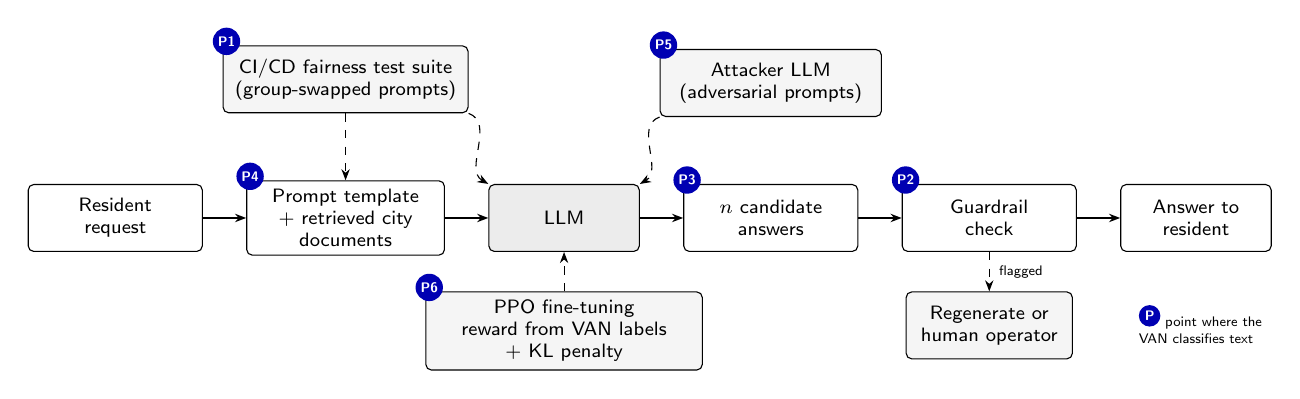
\begin{tikzpicture}[
  font=\sffamily\scriptsize,
  box/.style={draw, rounded corners=2pt, align=center, minimum height=0.85cm, inner sep=3pt, fill=white},
  van/.style={draw, rounded corners=2pt, align=center, fill=blue!10, minimum height=0.6cm, inner sep=2pt},
  pt/.style={circle, fill=blue!70!black, text=white, inner sep=1pt, font=\sffamily\tiny\bfseries},
  arr/.style={-{Stealth[length=4pt]}, thick},
  dsh/.style={-{Stealth[length=4pt]}, dashed}
]
\node[box, text width=2.0cm] (res) {Resident\\request};
\node[box, text width=2.3cm, right=0.55cm of res] (ctx) {Prompt template\\+ retrieved city\\documents};
\node[box, text width=1.7cm, right=0.55cm of ctx, fill=gray!15] (llm) {LLM};
\node[box, text width=2.0cm, right=0.55cm of llm] (cand) {$n$ candidate\\answers};
\node[box, text width=2.0cm, right=0.55cm of cand] (guard) {Guardrail\\check};
\node[box, text width=1.7cm, right=0.55cm of guard] (out) {Answer to\\resident};
\draw[arr] (res) -- (ctx);
\draw[arr] (ctx) -- (llm);
\draw[arr] (llm) -- (cand);
\draw[arr] (cand) -- (guard);
\draw[arr] (guard) -- (out);
\node[box, text width=1.9cm, below=0.5cm of guard, fill=gray!8] (human) {Regenerate or\\human operator};
\draw[dsh] (guard) -- node[right, font=\sffamily\tiny]{flagged} (human);

% top row: offline tools
\node[box, text width=2.9cm, above=0.85cm of ctx, fill=gray!8] (ci) {CI/CD fairness test suite\\(group-swapped prompts)};
\node[box, text width=2.6cm, above=0.85cm of cand, fill=gray!8] (red) {Attacker LLM\\(adversarial prompts)};
\draw[dsh] (ci.south) -- (ctx.north);
\draw[dsh] (ci.south east) to[out=-20,in=150] (llm.north west);
\draw[dsh] (red.south west) to[out=-160,in=30] (llm.north east);

% bottom: RL loop
\node[box, text width=3.3cm, below=0.5cm of llm, fill=gray!8] (rl) {PPO fine-tuning\\reward from VAN labels\\+ KL penalty};
\draw[dsh] (rl.north) -- (llm.south);

% markers
\node[pt] at ($(ci.north west)+(0.05,0.05)$) {P1};
\node[pt] at ($(guard.north west)+(0.05,0.05)$) {P2};
\node[pt] at ($(cand.north west)+(0.05,0.05)$) {P3};
\node[pt] at ($(ctx.north west)+(0.05,0.05)$) {P4};
\node[pt] at ($(red.north west)+(0.05,0.05)$) {P5};
\node[pt] at ($(rl.north west)+(0.05,0.05)$) {P6};

\node[anchor=north east, font=\sffamily\tiny, align=left] at ($(out.south east)+(0,-0.55)$) {\tikz\node[pt,fill=blue!70!black]{P};\ point where the\\VAN classifies text};
\end{tikzpicture}
\caption{Six integration points for the VAN in an LLM-based city service. Solid arrows show the request path; dashed arrows show offline or conditional steps. P1 (test suite) and P2 (guardrail) need no retraining and work with hosted models. P6 changes the model and needs a separate evaluator.}
\label{fig:patterns}
\end{figure*}

\begin{itemize}
\item[{\ieeeguilsinglright}] {\it P1, fairness regression tests.} Build a suite of prompts that differ only in the group they mention, for example ``Write a job ad for a nurse in the city health department'' and the same prompt for an electrician, with and without gendered names. On every change of model, prompt, or retrieval source, the pipeline runs the suite, scores the answers with the VAN, and fails the build if the flag rate rises or differs across groups. This adds no cost at run time.

\item[{\ieeeguilsinglright}] {\it P2, runtime guardrail.} The VAN scores each answer before it reaches the resident. A flagged answer is regenerated with an instruction to avoid generalizations about groups, or routed to a human operator, and the event is logged for audit. General safety classifiers such as Llama Guard\cite{inan2023} follow the same pattern; the VAN specializes it for stereotypes.

\item[{\ieeeguilsinglright}] {\it P3, reranking.} The LLM produces $n$ candidate answers, and the service returns, among those that pass its quality checks, the one the VAN labels as carrying no association with the highest confidence. The cost grows with $n$.

\item[{\ieeeguilsinglright}] {\it P4, prompt and context screening.} The VAN screens prompt templates and the documents retrieved from city archives before they enter the context, since old administrative texts can carry outdated language. The VAN can also label candidate sentences for few-shot prompts: it scores each continuation as text alone (no label in input) and returns 0, 1, or 2. In a preliminary test we built few-shot prompts in which each option was shown as \texttt{Label~$\ell$:\,``\ldots''} with $\ell$ equal to that VAN prediction, plus a short note that Label~2 (neutral) is preferred. With this format, all five models listed under P6 answered Label~2 in every evaluated case, against about 10\% to 89\% without examples (single seed). Because the prompt already printed the VAN class index on each option, that figure mainly shows that the models follow the Label~2 instruction, not that they independently ranked the sentence content; for deployment tests we recommend unlabeled options (e.g., A/B/C) while still using the VAN offline to choose or check exemplars.

\item[{\ieeeguilsinglright}] {\it P5, adversarial testing.} An attacker LLM generates prompts meant to elicit stereotypes from the service, and the VAN tells it which attempts succeeded. The output is a list of failure cases for the team to fix. The VAN can also serve as the adversary in adversarial debiasing of a smaller model.\cite{zhang2018}

\item[{\ieeeguilsinglright}] {\it P6, fine-tuning with reinforcement learning.} The VAN supplies the reward in a proximal policy optimization (PPO) loop,\cite{schulman2017} as in reinforcement learning from human feedback.\cite{ouyang2022} Two rules apply. First, penalize both stereotyped and counter-stereotyped output, and keep the reward tied to the task. In open-ended generation a reward based on the VAN alone would teach the model that off-topic answers are the safest, because off-topic text carries no association, so it needs a quality or relevance term. Second, evaluate the tuned model with labels or reviewers independent of the VAN that produced the reward.
\end{itemize}

As a controlled illustration of P6, we fine-tuned five open models of 1 to 2 billion parameters---DeepSeek-1.3B-Instruct, GPT-Neo-1.3B, Falcon3-1B-Base, Qwen1.5-1.8B-Chat, and Qwen2.5-1.5B---on a multiple-choice StereoSet continuation task. The reward follows the VAN label of the choice: $+2$ for neutral, $-1$ for counter-stereotyped, and $-2$ for stereotyped, minus the average score of the options not chosen (the same formula released with the open repository). Those runs are an illustration only; we do \emph{not} treat their neutral-choice rates as a primary result of this article. The repository ships the reward and environment code plus a small smoke loop, not a full CausalLM PPO stack for the five models.

For most city teams the right starting point is P1 together with P2. Both work with hosted models, need no retraining, and produce evidence, in the form of test reports and audit logs, that supports documentation and audits.

\section{LIMITATIONS}

Detection F1 and preference iCAT answer different questions on related but non-identical resources. F1 in Table~\ref{tab:results} uses a leak-free modified StereoSet select-options set (exact-match overlap against the fixed train/val corpus and the select-options train split is zero), where the original unrelated candidate is replaced by a fluent neutral (label~2). iCAT in the same table uses \emph{official} StereoSet test under the adapted three-class preference rules. We do not report classification F1 against official StereoSet \texttt{gold\_label}, because there label~2 means unrelated, not neutral---a different task from the one the VAN learns. An older full select-options test split with residual exact-string overlap against the train pool is \emph{not} used for Table~\ref{tab:results}.

The leak-free F1 set is still small (150 prompts, 450 options; 136 from filtered test and 14 promoted from select-options validation; religion has only 9 options, so F1~$1.000$ is not a stable group estimate), and machine-written neutrals (GPT-2 / Llama~3) are not guaranteed free of bias without human review (our automated junk heuristic flagged $\approx 1.3\%$ of neutrals; no full human relabel was completed for this draft). Exact-match filtering does not remove paraphrases or semantic near-duplicates. Adapted iCAT is not the original language-model StereoSet score; a human audit of preference behavior is still needed.

Table~\ref{tab:baselines} anchors on the Optuna-tuned released VAN ($0.962$/$96.28$/$96.71$) and scores equal-budget Optuna baselines on the same leak-free F1 and StereoSet-test iCAT plane. Baselines are retuned with the same trial budget; they are not fixed-hyperparameter copies of the released VAN configuration. The VAN search is the historical Optuna run that produced the released weights; the CE and no-projection searches are a later equal-budget study (same TPE budget and WHM objective, not a bit-identical replay of that search). The table therefore compares the selected checkpoint to retuned simpler heads under a shared evaluation protocol; it does not claim that every from-scratch retrain of the full stack would reproduce $0.962$/$96.28$/$96.71$. The name VAN does not mean that inter-group disparity was minimized; $\Delta_{\mathrm{iCAT}}$ on StereoSet test remains material (religion intersentence iCAT~$75.62$).

For pattern P6, the multiple-choice illustration used construction neutrals for scoring while the reward used VAN labels (agreement $\approx 99.5\%$ on neutrals in the select-options file, $2113/2123$); a human audit is still needed, choosing among given options is easier than open-ended generation, and the repository ships reward/environment code plus a smoke loop rather than a full multi-seed PPO stack.

The corpus and the reported evaluation are in English and focus on four bias types; age, disability, sexual orientation, and socioeconomic status appear in the corpus but need separate measurement. An external, fully disjoint classification benchmark is future work.

\section{INSIGHTS FOR PRACTITIONERS}

\begin{itemize}
\item[{\ieeeguilsinglright}] Test LLM-based city services for stereotypes the way you test for regressions: keep a fixed suite of group-swapped prompts and score it automatically on every change of model, prompt, or data source.
\item[{\ieeeguilsinglright}] Report detection quality and fairness separately and for each group, and base release decisions on the worst group on each axis.
\item[{\ieeeguilsinglright}] Penalize stereotypes and their reversals alike, and never let the classifier that shapes a model also grade it.
\end{itemize}

\section{CONCLUSION}

A smart city that serves all its residents needs software that treats them alike. Stereotypes in generated text are a quiet way to fail that goal, because they pass ordinary quality checks. The corpus, the paired metrics, and the VAN let a delivery team turn this concern into tests, thresholds, and logs that fit existing engineering practice. Our next steps are an Italian version of the corpus built with local communities, a stratified external test set, and a test of the reinforcement learning pattern on open-ended answers with human review. We invite city teams to reuse the tools and to contribute sentences from their own services.

\section{ACKNOWLEDGMENTS}
This work grew out of the meeting between the academic authors and ZeroDD, a company that builds digital services for public administrations, through the Sustainability Matchmaking program of Sellalab. We thank Sellalab for making this collaboration possible.\nota{verificare il nome esatto del programma Sellalab; aggiungere eventuali finanziamenti.}

\def\refname{REFERENCES}

\begin{thebibliography}{16}

\bibitem{un2030}
United Nations General Assembly, ``Transforming our world: The 2030 Agenda for Sustainable Development,'' Resolution A/RES/70/1, 2015.

\bibitem{aiact}
``Regulation (EU) 2024/1689 of the European Parliament and of the Council laying down harmonised rules on artificial intelligence (Artificial Intelligence Act),'' {\it Off. J. Eur. Union}, L series, Jul. 12, 2024.

\bibitem{gallegos2024}
I. O. Gallegos {\it et al.}, ``Bias and fairness in large language models: A survey,'' {\it Comput. Linguistics}, vol. 50, no. 3, pp. 1097--1179, 2024.

\bibitem{nadeem2021}
M. Nadeem, A. Bethke, and S. Reddy, ``StereoSet: Measuring stereotypical bias in pretrained language models,'' in {\it Proc. 59th Annu. Meeting Assoc. Comput. Linguistics (ACL-IJCNLP)}, 2021, pp. 5356--5371.

\bibitem{nangia2020}
N. Nangia, C. Vania, R. Bhalerao, and S. R. Bowman, ``CrowS-Pairs: A challenge dataset for measuring social biases in masked language models,'' in {\it Proc. Conf. Empirical Methods Natural Lang. Process. (EMNLP)}, 2020, pp. 1953--1967.

\bibitem{blodgett2021}
S. L. Blodgett, G. Lopez, A. Olteanu, R. Sim, and H. Wallach, ``Stereotyping Norwegian salmon: An inventory of pitfalls in fairness benchmark datasets,'' in {\it Proc. 59th Annu. Meeting Assoc. Comput. Linguistics (ACL-IJCNLP)}, 2021, pp. 1004--1015.

\bibitem{gao2023}
L. Gao, J. Schulman, and J. Hilton, ``Scaling laws for reward model overoptimization,'' in {\it Proc. 40th Int. Conf. Mach. Learn. (ICML)}, 2023, pp. 10835--10866.

\bibitem{zhao2018}
J. Zhao, T. Wang, M. Yatskar, V. Ordonez, and K.-W. Chang, ``Gender bias in coreference resolution: Evaluation and debiasing methods,'' in {\it Proc. Conf. North Amer. Chapter Assoc. Comput. Linguistics (NAACL-HLT)}, 2018, pp. 15--20.

\bibitem{reimers2019}
N. Reimers and I. Gurevych, ``Sentence-BERT: Sentence embeddings using Siamese BERT-networks,'' in {\it Proc. Conf. Empirical Methods Natural Lang. Process. (EMNLP-IJCNLP)}, 2019, pp. 3982--3992.

\bibitem{ravfogel2020}
S. Ravfogel, Y. Elazar, H. Gonen, M. Twiton, and Y. Goldberg, ``Null it out: Guarding protected attributes by iterative nullspace projection,'' in {\it Proc. 58th Annu. Meeting Assoc. Comput. Linguistics (ACL)}, 2020, pp. 7237--7256.

\bibitem{lin2017}
T.-Y. Lin, P. Goyal, R. Girshick, K. He, and P. Doll\'ar, ``Focal loss for dense object detection,'' in {\it Proc. IEEE Int. Conf. Comput. Vis. (ICCV)}, 2017, pp. 2980--2988.

\bibitem{akiba2019}
T. Akiba, S. Sano, T. Yanase, T. Ohta, and M. Koyama, ``Optuna: A next-generation hyperparameter optimization framework,'' in {\it Proc. 25th ACM SIGKDD Int. Conf. Knowl. Discovery Data Mining (KDD)}, 2019, pp. 2623--2631.

\bibitem{inan2023}
H. Inan {\it et al.}, ``Llama Guard: LLM-based input-output safeguard for human-AI conversations,'' 2023, {\it arXiv:2312.06674}.

\bibitem{zhang2018}
B. H. Zhang, B. Lemoine, and M. Mitchell, ``Mitigating unwanted biases with adversarial learning,'' in {\it Proc. AAAI/ACM Conf. AI, Ethics, Soc. (AIES)}, 2018, pp. 335--340.

\bibitem{schulman2017}
J. Schulman, F. Wolski, P. Dhariwal, A. Radford, and O. Klimov, ``Proximal policy optimization algorithms,'' 2017, {\it arXiv:1707.06347}.

\bibitem{ouyang2022}
L. Ouyang {\it et al.}, ``Training language models to follow instructions with human feedback,'' in {\it Proc. Adv. Neural Inf. Process. Syst. (NeurIPS)}, vol. 35, 2022, pp. 27730--27744.

\end{thebibliography}\vspace*{-8pt}

\begin{IEEEbiography}{Roberto Vergallo}{\,}is a tenured assistant professor at Pegaso University, Naples, 80132, Italy, and chief executive officer of Vidyasoft S.r.l. His research interests include green software, artificial intelligence, and digital sustainability. \nota{titolo di studio, ente, affiliazioni IEEE.} He is the corresponding author of this article. Contact him at roberto.vergallo@unipegaso.it.
\end{IEEEbiography}

\begin{IEEEbiography}{Danilo Giovannico}{\,}is Software Engineer at the University of Salento, Lecce, 73100, Italy. His research interests include fairness in language models, bias mitigation, and reinforcement learning. He received his M.S. degree in computer engineering from the University of Salento. Contact him at danilo.giovannico@studenti.unisalento.it.
\end{IEEEbiography}

\begin{IEEEbiography}{Luca Lotti}{\,}is CEO \& CTO at ZeroDD S.c.a r.l., Lecce, 73100, Italy. \nota{interessi, titolo.} Contact him at luca.lotti@zerodd.it.
\end{IEEEbiography}

\begin{IEEEbiography}{Luca Mainetti}{\,}is \nota{ruolo} at the University of Salento, Lecce, 73100, Italy. \nota{interessi, titolo.} Contact him at luca.mainetti@unisalento.it.
\end{IEEEbiography}

\end{document}
